% Acciones y transiciones de estado del modelo sin giro (GridRobotNotTurning).
\providecommand{\ejeH}{c}
\providecommand{\ejeV}{r}
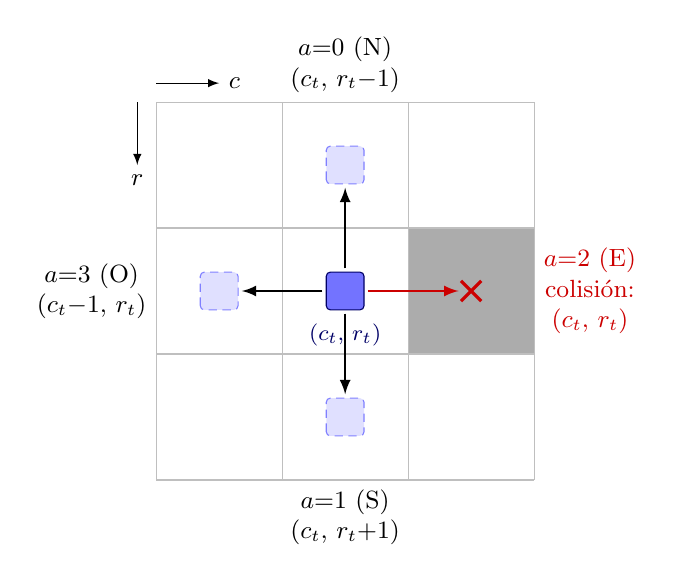
\begin{tikzpicture}[scale=1.6, >=latex,
        robot/.style={fill=blue!55, draw=blue!40!black, rounded corners=1.5pt},
        destino/.style={fill=blue!12, draw=blue!50, densely dashed, rounded corners=1.5pt},
        accion/.style={font=\small, align=center}]
    \fill[gray!65] (2,1) rectangle (3,2);
    \draw[gray!50] (0,0) grid (3,3);
    % Ejes de la rejilla (origen arriba a la izquierda)
    \draw[->] (0,3.15) -- (0.5,3.15) node[right] {\small $\ejeH$};
    \draw[->] (-0.15,3) -- (-0.15,2.5) node[below] {\small $\ejeV$};
    % Posiciones alcanzables
    \draw[destino] (1.35,2.35) rectangle (1.65,2.65);
    \draw[destino] (1.35,0.35) rectangle (1.65,0.65);
    \draw[destino] (0.35,1.35) rectangle (0.65,1.65);
    % Robot en el estado actual
    \draw[robot] (1.35,1.35) rectangle (1.65,1.65);
    \node[font=\footnotesize, text=blue!40!black] at (1.5,1.15) {$(\ejeH_t,\,\ejeV_t)$};
    % Acciones
    \draw[->, thick] (1.5,1.68) -- (1.5,2.32);
    \draw[->, thick] (1.5,1.32) -- (1.5,0.68);
    \draw[->, thick] (1.32,1.5) -- (0.68,1.5);
    \draw[->, thick, red!80!black] (1.68,1.5) -- (2.4,1.5);
    \draw[red!80!black, very thick] (2.42,1.42) -- (2.58,1.58)
        (2.42,1.58) -- (2.58,1.42);
    % Acción y estado resultante
    \node[accion, above] at (1.5,3) {$a{=}0$ (N)\\ $(\ejeH_t,\,\ejeV_t{-}1)$};
    \node[accion, below] at (1.5,0) {$a{=}1$ (S)\\ $(\ejeH_t,\,\ejeV_t{+}1)$};
    \node[accion, left] at (0,1.5) {$a{=}3$ (O)\\ $(\ejeH_t{-}1,\,\ejeV_t)$};
    \node[accion, right, text=red!80!black] at (3,1.5)
        {$a{=}2$ (E)\\ colisión:\\ $(\ejeH_t,\,\ejeV_t)$};
\end{tikzpicture}
